%% APPENDIX B -- the spatial rank as a diagnostic: what it can and cannot
%% support, and the reserved hold-out that calibrates it.
%% Owner: r11-chain.  Carries \label{app:radius} (cited by 04_method.tex)
%% and \label{sec:heldout} (cited from the other appendices)
%% and \label{sec:nullscatter} (v4.23: cited by 05_results.tex's
%% false-alarm sentence, which quotes the MEASURED scatter of this very
%% null -- the reference used to read `app:spatialnorm`, a label that has
%% never existed in this tree and which stopped the build at `labelcheck`).
\section{The spatial rank, and what it can support}
\label{app:radius}

The spatial rank asks whether an excess sits at the star or anywhere else in
the field. It is a diagnostic on which no disposition rests
(\S\ref{sec:summary}). The star lies near the phase centre, inside the control
annulus, and carries more above-threshold cells than a control position at
every level below the trigger (Appendix~\ref{app:falsealarm}). \emph{This is
not a primary-beam effect}: spectra are extracted in apparent flux density
from phase-rotated visibilities (Appendix~\ref{app:conventions}), and a noise
rise toward the field edge would put the stellar rank \emph{above} one half,
the opposite of what is measured. The ensemble's own weak rise with radius is
removed by standardising each probe within its radius bin
(\texttt{documentation/\allowbreak appendix\_B\_spatial\_normalisation.md} of
the data archive, \citealt{SIdeposit}).

A calibration error that varied with frequency -- a bandpass residual, or a
coarse-mode system temperature interpolated near a telluric line
\citep{ALMATsys2018} -- multiplies the continuum, so it would act at the star
and not on empty sky, with the sign observed. \emph{Its amplitude is too
small.} A fractional error $\epsilon$ reaches the trigger only if
$\epsilon=5\sigma/S_{\rm c}$, with the continuum $S_{\rm c}$ measured for
\CyNWinMeas{} of the \CyNWinTot{} windows. No window requires as little as the
\CySpecTsysLo--\CySpecTsysHi{} per cent a coarse system temperature leaves at
an ozone line: the least anywhere is \CyEpsMinPct{} per cent and the median
\CyEpsMedPct. The bandpass branch needs $\CyMarginBp\times$ the
\CdSpecBpWorst{} per cent quoted for the worst bands
\citep{ALMAKBBandpass,ALMATechNote15}.

An additive visibility error (a correlator offset, cross-talk or coherent
interference) images at the phase centre, where the star sits and the annulus
does not. The excess is not confined there: the ratio is \BgPcOnRatio{}
(\BgPcOnRatioLo--\BgPcOnRatioHi) in the \BgPcOnNWin{} windows with the star
within one synthesised beam of the phase centre and \BgPcOffRatio{}
(\BgPcOffRatioLo--\BgPcOffRatioHi) in the \BgPcOffNWin{} beyond it, with
\BgPcOnObs{} and \BgPcOffObs{} unattributed crossings against \BgPcOnExp{} and
\BgPcOffExp{} expected. The outer set (\BgPcOffTopN{} of its windows toward
\BkAlmaName) is too small to exclude a contribution. The excess appears only
in the 7\,m-array data, \BgArrSevenRatio{}
(\BgArrSevenRatioLo--\BgArrSevenRatioHi) against \BgArrTwelveRatio{}
(\BgArrTwelveRatioLo--\BgArrTwelveRatioHi) on the 12\,m array, and its cause is
not identified.

\subsection{The reserved hold-out, and what it calibrates}
\label{sec:heldout}

The statistic and the mask are set on the searched sample and cannot
calibrate themselves, so a further sample is held out by an identifier rule,
$\mathrm{sha256}(\textsc{uid})_{[:8]} \bmod 5 = 0$, with two guards using
identifiers alone: a block on a named list stays in the survey, and no system
loses every block. Its independence of the statistic and the mask is our
assertion, not something a reader can check. \NEbHeldOut{} of
\NEbProcessedAll{} blocks are reserved, \HoWin{} windows toward \HoStars{}
stars. Because the rule hashes the block and not the session, \HsSharePct{}
per cent of the reserved set shares calibrators, weather and setup with a
searched block -- a session-level hash would have been stronger -- so every
quantity from it is also given over the \HsIndBlocks{} blocks that share no
session.

\subsection{The recurrence statistic under the null}
\label{sec:nullscatter}

The bound in the crossing ledger is one formula. Writing $S$ and
$\sigma_{\rm d}$ for the discovery amplitude and its error, and $\bar{a}$ and
$\bar{\sigma}=(\sum_i\sigma_i^{-2})^{-1/2}$ for the inverse-variance
combination of the repeat readings at the predicted channel,
\begin{equation}
\sigma_{\rm excl}=\frac{S-\bar{a}}
{\sqrt{\sigma_{\rm d}^{2}+\bar{\sigma}^{2}}}
=\frac{T_{\rm pers}-T_{\rm rep}}{\sqrt{1+(T_{\rm pers}/T_\star)^{2}}},
\label{eq:excl}
\end{equation}
with $T_{\rm pers}=S/\bar{\sigma}$ and $T_{\rm rep}=\bar{a}/\bar{\sigma}$, so
every bound follows from Eq.~\ref{eq:excl} and three columns of that table.
$T_{\rm rep}$ is one cell at the carried drift. The maximum over every drift
at that cell is tabulated beside it but never compared with $T_{\rm pers}$:
it is positive on average whatever is there. As an amplitude selected from
$10^{\TuCellsDecLo}$ to $10^{\TuCellsDecHi}$ cells at $T_\star\simeq5$ is
biased high, the limit is stated as $(T_{\rm rep}+5)/T_{\rm pers}$. The
reading is centred on zero, scattering by \NuNullSd{} about \NuNullMean{} over
\NuNullN{} single-cell readings of every repeat block in the census and
hold-out, less the \NuNullNRecExcl{} of the crossing that recurs, a molecular
line. The bound's power is $\Phi(T_{\rm pers}-5)$ at the discovery amplitude
and $\Phi(5T_{\rm pers}/T_\star-5)$ at the trigger amplitude $5S/T_\star$, the
faintest that could have produced the crossing; the \HjNPowerLo{} where these
are smallest are reported as untested. Each crossing's measured recovery
chance accompanies this paper as data.

%% fig:bpiccontrol belongs here, where the spatial statistic is characterised.
\begin{figure}
\centering
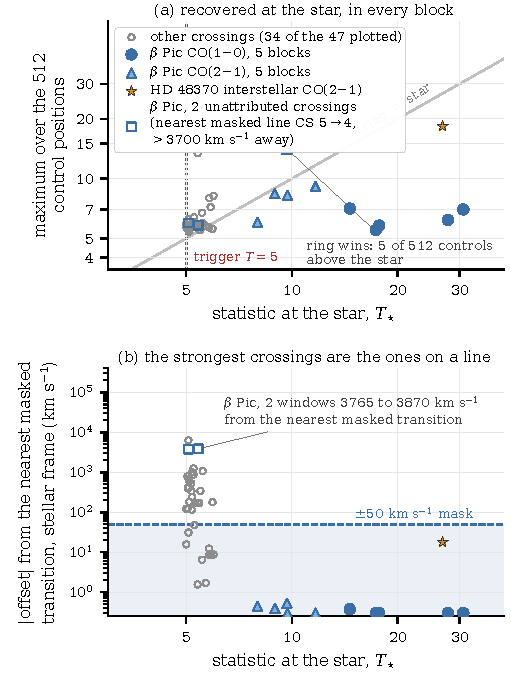
\includegraphics[width=\columnwidth]{figures/bpic_control.pdf}
\caption{The $\beta$~Pictoris positive control.
\emph{(a)}~Stellar statistic against the maximum over the window's \NCtrl{}
control positions, filled for blocks recovering its CO.
\emph{(b)}~Offset from the nearest masked transition in the star's own frame,
$\pm\MaskHalfKms$\,km\,s$^{-1}$ marked: its \BpicPanelNCo{} CO crossings lie
\BpicDvCoLo--\BpicDvCoHi\,km\,s$^{-1}$ from CO, its \BpicPanelNCs{}
unattributed ones \BpicDvCsLo--\BpicDvCsHi\,km\,s$^{-1}$ from any; grey, the other
quality-passing crossings.}
\label{fig:bpiccontrol}
\end{figure}
